\documentclass[10pt,a4paper]{article}
\usepackage[margin=2.3cm]{geometry}
\usepackage{amsmath,amssymb}
\usepackage{graphicx}
\usepackage{booktabs}
\usepackage{listings}
\usepackage{xcolor}
\usepackage[colorlinks=true,linkcolor=blue!50!black,citecolor=blue!50!black,urlcolor=blue!50!black]{hyperref}

\lstset{basicstyle=\ttfamily\small,columns=fullflexible,keepspaces=true,
        backgroundcolor=\color{gray!8},frame=single,rulecolor=\color{gray!40},
        xleftmargin=4pt,xrightmargin=4pt,aboveskip=6pt,belowskip=6pt,
        breaklines=true,breakatwhitespace=true}
\newcommand{\cmd}[1]{\texttt{#1}}
\setlength{\emergencystretch}{3em}

\title{\textbf{BondFlux}\\[2pt]\large A simulation toolkit for dynamic bonds in polymer networks\\[2pt]
\normalsize \texttt{fix bond/flux} for LAMMPS --- user manual and validation}
\author{}
\date{October 2026}

\begin{document}
\maketitle

\noindent
BondFlux simulates polymer networks whose bonds can form, break, and exchange. It is a single
LAMMPS fix style, \cmd{fix bond/flux}, with two modes: Monte Carlo (MC) moves of topological bonds
(\cmd{mc}), and the Sciortino three-body swap potential (\cmd{3body}). This manual explains the two
methods, the LAMMPS commands, how to add the fix to LAMMPS, and the tests that validate it.

\tableofcontents

%======================================================================
\section{Introduction}

Dynamic covalent and supramolecular bonds let a polymer network change its topology while it is
deformed or heated. In associative networks (vitrimers) bonds exchange partners at a constant number
of cross-links~\cite{Montarnal2011}. In dissociative networks bonds break and re-form, so their number
follows the temperature. In multiple-network elastomers, a pre-stretched filler network breaks
irreversibly under load while a permanent matrix keeps the material together~\cite{Ducrot2014}.
BondFlux handles all three in a coarse-grained model such as the Kremer--Grest bead-spring
model~\cite{Kremer1990}. Exchange, formation and breaking can be combined with each other and with
the irreversible scission of bonds through \cmd{bond\_style quartic}.

Two routes are used in the literature. In the first, a dynamic bond is an explicit LAMMPS bond, and
an MC step between MD steps changes the topology (Perego and Khabaz~\cite{Perego2020},
Xia and Olvera de la Cruz~\cite{Xia2023}, and others). In the second, a bond is a
short-ranged pair attraction. A three-body repulsion enforces one bond per sticker and makes the
bond swap barrier-free, so standard MD produces the exchange~\cite{Sciortino2017}. BondFlux provides
both routes in the same fix (Table~\ref{tab:modes}).

\begin{table}[h]
\centering
\caption{The two modes of \cmd{fix bond/flux}.}\label{tab:modes}
\small
\begin{tabular}{lll}
\toprule
 & \cmd{mc} & \cmd{3body} \\
\midrule
dynamic bond & LAMMPS bond of one type & pair interaction within $r_c$ \\
topology changes by & Metropolis MC every $N$ steps & MD (continuous forces) \\
moves & shift, swap, formation, breaking & swap, thermal breaking and formation \\
number of bonds & conserved, or fluctuating with \cmd{form}/\cmd{break} & fluctuating (fixed if $\epsilon\gg kT$) \\
rate control & attempt gate $e^{-E_a/kT}$, frequency & $\lambda$, temperature \\
\bottomrule
\end{tabular}
\end{table}

\subsection{Monte Carlo moves of topological bonds}

The atoms of the fix group are \emph{stickers}. Each sticker has at most one dynamic bond, a LAMMPS
bond of the type \cmd{btype}. Every $N$ steps each sticker is visited once and offered one move
(Fig.~\ref{fig:moves}):
\begin{itemize}
\item a bonded sticker $i$ with partner $k$ breaks the bond with probability $p_b$ (\cmd{break}),
  and otherwise attempts an exchange with a candidate $j$, chosen uniformly among the stickers
  within the reaction window of $i$:
  a \emph{shift} $i$--$k$ + $j$ $\to$ $i$--$j$ + $k$ if $j$ is free,
  or a \emph{swap} $i$--$k$ + $j$--$l$ $\to$ $i$--$j$ + $k$--$l$ if $j$ is bonded to $l$;
\item a free sticker $i$ forms a bond with probability $p_f$ (\cmd{form}), with a free candidate
  $j$ chosen uniformly.
\end{itemize}
Every bond that is broken \emph{or} formed must have a length in the reaction window
$[r_\text{min}, r_c)$. This rule makes each move reversible from the same sticker with the same
proposal probability: in a shift, the free stickers near $i$ before the move are the free stickers
near $i$ after it, with $j$ and $k$ exchanged, and both are inside the window. Candidates must be
bondable (\cmd{bondable} types, \cmd{molecule} rule) and must not already be bonded to $i$ through
another bond.

\begin{figure}[h]
\centering
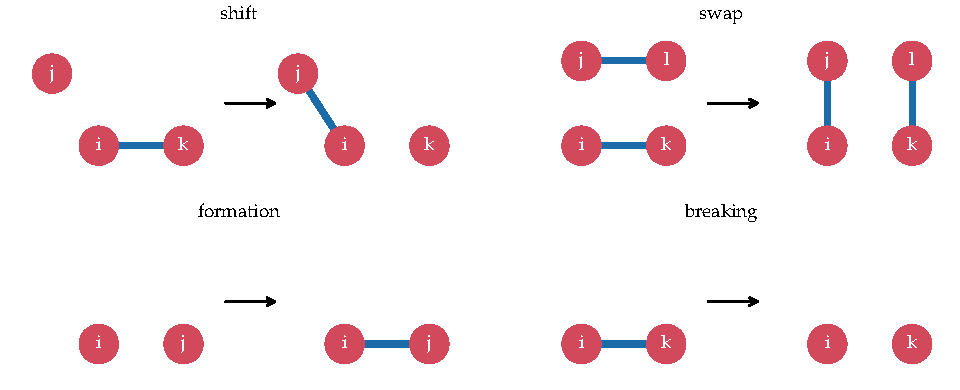
\includegraphics[width=0.95\textwidth]{figures/moves.pdf}
\caption{Monte Carlo moves of \cmd{fix bond/flux mc}: sticker $i$ is the sticker offered the move;
dynamic bonds are drawn as lines. Exchange (shift, swap) keeps the number of dynamic bonds; formation
and breaking change it.}\label{fig:moves}
\end{figure}

\paragraph{Energy change.}
The energy change of a move is evaluated with the bond and pair styles of the simulation:
\begin{equation}
\Delta E = \sum_\text{formed} \bigl[U_\text{bond}(r) - \Delta U_\text{pair}(r)\bigr]
         - \sum_\text{broken} \bigl[U_\text{bond}(r) - \Delta U_\text{pair}(r)\bigr]
         + E_\text{bond}\,(n_\text{formed} - n_\text{broken}),
\end{equation}
where $\Delta U_\text{pair}(r) = U_\text{pair}(r;1) - U_\text{pair}(r;w_{12})$ is the change of the
pair energy when a pair stops being a 1--2 neighbor ($w_{12}$ = \cmd{special\_bonds} weight) and
$E_\text{bond}$ is an optional association energy (\cmd{ebond}). For a Kremer--Grest model with
\cmd{special\_bonds lj 0 1 1}, a FENE bond and a WCA pair, the WCA terms cancel and
$\Delta E$ is the change of the FENE energy; with \cmd{special\_bonds 1 1 1} (required by
\cmd{bond\_style quartic}) $\Delta U_\text{pair}=0$. $\Delta E$ is exactly the change of the
LAMMPS potential energy, as checked in Sec.~\ref{sec:tests}.

\paragraph{Acceptance.}
Exchange moves are accepted with $\min(1, e^{-\Delta E/kT})$. Formation and breaking are each
other's reverse but are proposed with different probabilities (a free sticker picks one of $n_c$
candidates; a bonded sticker breaks with probability $p_b$), so they carry the Metropolis--Hastings
ratio
\begin{equation}
P_\text{form} = \min\Bigl(1, \frac{p_b\, n_c}{p_f}\, e^{-\Delta E/kT}\Bigr), \qquad
P_\text{break} = \min\Bigl(1, \frac{p_f}{p_b\, n_c'}\, e^{-\Delta E/kT}\Bigr),
\end{equation}
where $n_c'$ is the number of free candidates of $i$ after the bond is broken.

\paragraph{Barrier.}
A reaction barrier $E_a$ (\cmd{barrier}) and an attempt probability $P$ (\cmd{prob}) enter as a
gate: a sticker is offered a move only with probability $g = P\,e^{-E_a/kT}$. The gate multiplies the
rate of every move and of its reverse by the same factor, so it changes the kinetics and leaves the
equilibrium unchanged (Sec.~\ref{sec:rules}). Adding $E_a$ to $\Delta E$ inside the Metropolis
exponent, as in Ref.~\cite{Xia2024b}, does not have this property.

\paragraph{Parallel moves.}
A move centered on sticker $i$ involves atoms within $2r_c$ of $i$. Each MPI sub-domain is split
into $2^d$ sectors, and the sectors are processed one after the other; moves in the same sector of
neighboring processors are then at least half a sub-domain apart and cannot conflict. Partner
changes of ghost atoms are sent to their owners after each sector, also through the multi-hop paths
near sub-domain corners. At the end of an MC step the bond and 1--2 special lists are updated and a
reneighboring is triggered. The partner bookkeeping is rebuilt from the bond list at every MC step,
so bonds broken by \cmd{bond\_style quartic} are picked up automatically.

\subsection{Three-body swap potential}

In \cmd{3body} mode the fix adds the Sciortino potential~\cite{Sciortino2017} between bondable
stickers. The two-body bond is a $2n$--$n$ Lennard-Jones potential,
\begin{equation}
V(r) = \epsilon\,\frac{\phi(r) - \phi(r_c)}{1 + \phi(r_c)}, \qquad
\phi(r) = 4\Bigl[\Bigl(\frac{\sigma}{r}\Bigr)^{2n} - \Bigl(\frac{\sigma}{r}\Bigr)^{n}\Bigr],
\qquad r < r_c,
\end{equation}
shifted to zero at $r_c$ and rescaled to a depth of $-\epsilon$ at $r_\text{min} = 2^{1/n}\sigma$.
With \cmd{eshift no}, $V = \epsilon\,\phi(r)$ is used unshifted, as in HOOMD-blue's RevCross. The
three-body term,
\begin{equation}
E_3 = \lambda\,\epsilon \sum_i \sum_{j<k} V_3(r_{ij})\,V_3(r_{ik}), \qquad
V_3(r) = \begin{cases} 1 & r \le r_\text{min}\\ -V(r)/\epsilon & r_\text{min} < r < r_c\end{cases},
\end{equation}
penalizes a sticker with two partners. For $\lambda = 1$ the energy gained by a second partner is
compensated exactly, so the swap is barrier-free; $\lambda > 1$ adds an exchange barrier of
$(\lambda - 1)\epsilon$. Forces, energy and virial are computed in the \cmd{pre\_reverse} stage on a
full neighbor list, and forces on ghost atoms are summed by LAMMPS's reverse communication. The fix
supplies the complete interaction between bondable sticker types; the pair style interaction
between them must be switched off (\cmd{pair\_coeff A B 0.0 ...}).

The three-body potential is widely used for coarse-grained vitrimers, for example by Liu,
Ganesan and co-workers to relate the bond swap barrier to the structure, mechanics, self-healing
and reprocessing of vitrimer networks~\cite{Zhao2022}, and by Sing and co-workers to study
penetrant diffusion in vitrimer networks~\cite{Lin2026}.

%======================================================================
\section{Using fix bond/flux in LAMMPS}

\subsection{Syntax}
\begin{lstlisting}
fix ID group-ID bond/flux mc    Nevery btype rc T seed keyword value ...
fix ID group-ID bond/flux 3body eps sigma n rc lambda keyword value ...
\end{lstlisting}
\begin{itemize}
\item \cmd{mc}: \cmd{Nevery} = steps between MC steps; \cmd{btype} = bond type of the dynamic bonds;
  \cmd{rc} = upper end of the reaction window (distance); \cmd{T} = temperature of the Metropolis
  test (use the thermostat set point); \cmd{seed} = random number seed.
\item \cmd{3body}: \cmd{eps}, \cmd{sigma}, \cmd{n} = depth, size and exponent of the $2n$--$n$ bond;
  \cmd{rc} = cutoff; \cmd{lambda} = three-body strength.
\end{itemize}

\begin{table}[h]
\centering
\caption{Keywords.}\label{tab:keywords}
\begin{tabular}{llll}
\toprule
keyword & mode & value & default \\
\midrule
\cmd{bondable} & both & \cmd{itype jtype} (ranges allowed, repeatable) & all pairs \\
\cmd{shift}, \cmd{swap} & mc & \cmd{yes}/\cmd{no} & \cmd{yes} \\
\cmd{form}, \cmd{break} & mc & attempt probabilities $p_f$, $p_b$ (both $>0$ or both 0) & 0, 0 \\
\cmd{ebond} & mc & association energy per dynamic bond & 0 \\
\cmd{barrier} & mc & activation energy $E_a$ & 0 \\
\cmd{prob} & mc & attempt probability $P$ & 1 \\
\cmd{rmin} & mc & lower end of the reaction window & 0 \\
\cmd{molecule} & mc & \cmd{any}, \cmd{inter}, \cmd{intra} & \cmd{any} \\
\cmd{rbond} & 3body & distance that defines a bond for the output & \cmd{rc} \\
\cmd{eshift} & 3body & \cmd{yes}/\cmd{no}: shift $V$ to zero at \cmd{rc} & \cmd{yes} \\
\bottomrule
\end{tabular}
\end{table}

\paragraph{Output.}
\cmd{mc}: global vector with 11 elements (attempts, proposals, accepted shifts, swaps,
formations, breakings, geometric rejections, Metropolis rejections, sum of $\Delta E$ of accepted
moves, number of dynamic bonds, accepted moves in the last MC step); global scalar
$E_\text{bond}\times$(number of dynamic bonds) when \cmd{ebond} is set, included in the potential
energy. \cmd{3body}: global scalar = $E_2 + E_3$ (included in the potential energy and virial),
vector ($E_2$, $E_3$, bonded pairs, stickers with more than one partner). Per-atom array, both
modes: column 1 = partner atom ID (nearest bonded partner in \cmd{3body}), column 2 = number of
moves of the atom (\cmd{mc}) or number of partners within \cmd{rbond} (\cmd{3body}).

\paragraph{Restrictions.}
\cmd{mc}: molecular atom style; orthogonal box; \cmd{special\_bonds lj/coul $w_{12}$ 1.0 1.0}
(1--3 and 1--4 neighbors must not be special); \cmd{comm\_modify cutoff} $\ge 2r_c + \text{skin}/2$;
processor sub-domains $\ge 8r_c + \text{skin}$; \cmd{extra/bond/per/atom} and
\cmd{extra/special/per/atom} when bonds can form; angles or dihedrals must not contain dynamic bonds.
For FENE bonds $r_c < 0.95R_0$; for quartic bonds $r_c$ must be shorter than the breaking distance.
LAMMPS cannot combine \cmd{quartic} with unbreakable styles in \cmd{bond\_style hybrid}, so a network
with breakable quartic strands uses quartic dynamic bonds as well. \cmd{3body}: \cmd{newton on};
\cmd{comm\_modify cutoff} $\ge r_c + \text{skin}$. Neither mode supports \cmd{run\_style respa}.
The fix writes no restart data: after \cmd{read\_restart} it is defined again, the partners are
rebuilt from the bond list, and the per-atom move counts and random number streams start anew.

\subsection{Examples}

\paragraph{Kremer--Grest vitrimer} (exchange only, number of bonds conserved; \cmd{examples/kg\_network}):
\begin{lstlisting}
special_bonds   lj/coul 0.0 1.0 1.0
bond_style      fene
bond_coeff      * 30.0 1.5 1.0 1.0
group           stick type 2
fix             flux stick bond/flux mc 100 2 1.3 1.0 777 barrier 2.0
\end{lstlisting}

\paragraph{Dissociative network} (reversible formation and breaking with association energy):
\begin{lstlisting}
fix             flux stick bond/flux mc 100 2 1.3 1.0 12347 form 1.0 break 0.5 ebond -24.0
\end{lstlisting}

\paragraph{Multiple network with breakable strands} (quartic bonds; type 1 = permanent strands,
type 2 = dynamic junctions; strands break irreversibly above 1.3$\sigma$):
\begin{lstlisting}
special_bonds   lj/coul 1.0 1.0 1.0
bond_style      quartic
bond_coeff      1 1200.0 -0.55 0.25 1.3 34.6878
bond_coeff      2 1200.0 -0.55 0.25 1.3 34.6878
fix             flux stick bond/flux mc 10 2 1.2 1.0 4321 barrier 3.0
\end{lstlisting}

\paragraph{Cross-linker vitrimer as in Refs.~\cite{Xia2023,Xia2024b}} (A stickers on chains, B ends of
three-bead cross-linkers, LJ with $r_c = 1.5\sigma$, MC every 10 steps, reaction window
$0.87\le r < 1.14$; only free A stickers attack bonded B):
\begin{lstlisting}
special_bonds   lj/coul 0.0 1.0 1.0
bond_coeff      2 30.0 1.5 0.0 1.0      # FENE without the WCA term
fix             flux AB bond/flux mc 10 2 1.14 1.0 9876 bondable 1 2 swap no rmin 0.87 barrier ${Ub}
\end{lstlisting}

\paragraph{Pair-swap vitrimer as in Ref.~\cite{Perego2020}} (all stickers bonded, swaps only, an MC step
every MD step):
\begin{lstlisting}
fix             flux stick bond/flux mc 1 2 1.3 1.0 5555 shift no
\end{lstlisting}

\paragraph{Sciortino dumbbells} (\cmd{examples/dumbbells}; A--A and B--B repulsive $2n$--$n$ WCA):
\begin{lstlisting}
pair_style      mie/cut $(2.0^(1.0/100))
pair_coeff      * * 1.0 1.0 200 100
pair_coeff      1 2 0.0 1.0 200 100
pair_modify     shift yes
fix             tb stick bond/flux 3body 1.0 1.0 100 1.3 1.0 bondable 1 2
\end{lstlisting}
The model of Ref.~\cite{Lin2026} corresponds to \cmd{3body 30.0 1.0 100 1.2 lambda}.

%======================================================================
\section{Adding BondFlux to LAMMPS}

The fix uses only core LAMMPS classes and is compiled as part of the LAMMPS core. With CMake:
\begin{lstlisting}
cd lammps/src
ln -s ../../src/fix_bond_flux.h ../../src/fix_bond_flux.cpp .     # or copy the two files
cd ..
cmake -S cmake -B build -D PKG_MOLECULE=on -D PKG_EXTRA-PAIR=on -D BUILD_MPI=on -D BUILD_SHARED_LIBS=on
cmake --build build -j 8
build/lmp -h | grep bond/flux
\end{lstlisting}
\cmd{PKG\_MOLECULE} provides the bond styles, \cmd{PKG\_EXTRA-PAIR} the \cmd{mie/cut} pair style of
the dumbbell examples, and \cmd{BUILD\_SHARED\_LIBS} the library for the Python tests. With the
legacy make build, copy the two files into \cmd{lammps/src} and run \cmd{make mpi}. BondFlux was
developed and tested with LAMMPS stable 30 Sep 2026.

%======================================================================
\section{Validity tests}\label{sec:tests}

The scripts are in \cmd{tests/} and \cmd{examples/}; the figure data are in
\cmd{doc/data/bondflux\_validation.h5}.

\subsection{Exact detailed balance of the MC moves}

Six stickers are frozen in place (no time integration), so only the MC moves change the system.
The visited topologies must then follow $e^{-E/kT}$ over all topologies the moves can reach. The
reachable topologies and their energies are enumerated independently of LAMMPS
(\cmd{tests/test\_mc\_balance.py}). The test was run for four force fields: Kremer--Grest FENE with
\cmd{special\_bonds 0 1 1}; quartic with \cmd{1 1 1}; FENE without WCA, where bonded pairs lose
their repulsion; and harmonic with a 1--2 weight of 0.5. It covered exchange only, formation and
breaking only, and both together, with and without a barrier, on 1, 2 and 4 MPI ranks, with the
cluster in the middle of the box and across a periodic box corner. All 48 runs pass: the largest
block z-score is below 3.1, the total variation distance below 0.006, and the LAMMPS potential
energy changes by the sum of the $\Delta E$ of the accepted moves to $10^{-10}$.
Figure~\ref{fig:balance} shows the run with formation and breaking on 4 ranks.

\begin{figure}[h]
\centering
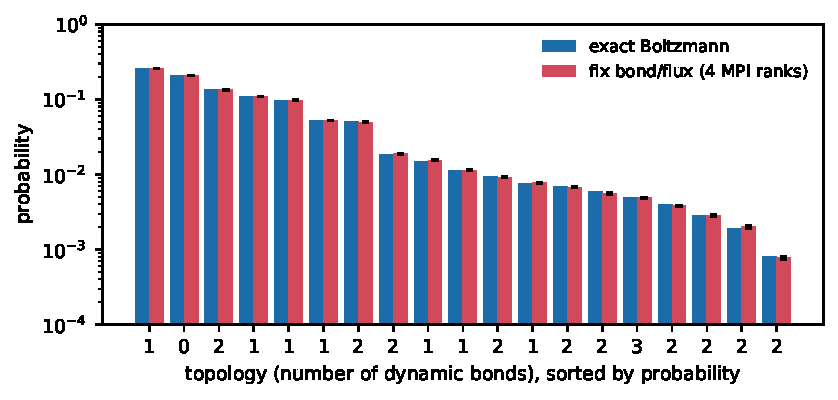
\includegraphics[width=0.85\textwidth]{figures/mc_balance.pdf}
\caption{Probabilities of the 19 reachable topologies of a frozen six-sticker cluster (0, 1 or 2
dynamic bonds) with exchange, formation and breaking ($p_f=p_b=0.5$, $E_\text{bond}=-20\epsilon$,
$kT=4\epsilon$, Kremer--Grest FENE, $4\times10^5$ MC steps on 4 MPI ranks) compared with the exact
Boltzmann distribution. Total variation distance 0.0018.}\label{fig:balance}
\end{figure}

\subsection{Barrier as a gate versus inside the Metropolis exponent}\label{sec:rules}

For the same cluster, the transition matrix of the exchange MC was built exactly and its stationary
distribution compared with the Boltzmann distribution (\cmd{tests/compare\_acceptance\_rules.py}).
With the gate of \cmd{fix bond/flux} the stationary distribution is Boltzmann for every barrier.
With the barrier added to $\Delta E$, a move and its reverse are both penalized, so for
$|\Delta E| < E_a$ their acceptance ratio becomes $e^{-2\Delta E/kT}$. The equilibrium of the
topology is then that of half the temperature (Table~\ref{tab:rules}).

\begin{table}[h]
\centering
\caption{Total variation distance between the stationary distribution and the Boltzmann
distribution (exact, no sampling). Gate: $P_\text{acc}=e^{-E_a/kT}\min(1,e^{-\Delta E/kT})$;
inside exponent: $P_\text{acc}=\min(1,e^{-(\Delta E+E_a)/kT})$.}\label{tab:rules}
\begin{tabular}{llccccc}
\toprule
rule & window & $E_a/kT=0$ & 1 & 2 & 4 & 8\\
\midrule
gate (BondFlux) & $[0,1.3)$ & $2\times10^{-15}$ & $2\times10^{-14}$ & $1\times10^{-14}$ & $1\times10^{-13}$ & $2\times10^{-11}$\\
inside exponent & $[0,1.3)$ & $2\times10^{-15}$ & 0.235 & 0.275 & 0.283 & 0.283\\
gate (BondFlux) & $[0.87,1.14)$ & $3\times10^{-17}$ & $6\times10^{-16}$ & $2\times10^{-15}$ & $1\times10^{-14}$ & $4\times10^{-13}$\\
inside exponent & $[0.87,1.14)$ & $3\times10^{-17}$ & 0.149 & 0.149 & 0.149 & 0.149\\
\bottomrule
\end{tabular}
\end{table}

\noindent A reaction window checked only for the new bond~\cite{Xia2023} is not reversible either: a
bond stretched beyond the window can be exchanged away but never formed. This bias acts through
bond-length fluctuations and does not appear for a frozen cluster.

\subsection{Three-body forces, virial and the HOOMD-blue implementation}

\cmd{tests/test\_3body.py} compares the forces with central finite differences of the total
energy, and the virial with finite-difference strain derivatives (box scaling in $x$, $y$, $z$ and
an $xy$ shear). The test uses $n=12$ and 100, $\lambda=1$ and 1.3, and 1, 2 and 4 MPI ranks. The
relative errors are $\le 8\times10^{-10}$ for the forces and $\le 3\times10^{-9}$ for the virial, and
the parallel forces agree with the serial ones to $2\times10^{-13}$. For an A--B bond at $r_\text{min}$
and a second B approaching from the other side, the total energy stays $-\epsilon$ to $10^{-12}$
while the two-body energy varies between $-2\epsilon$ and $-\epsilon$ ($n=100$, $\lambda = 1$).

\cmd{tests/test\_hoomd\_revcross.py} runs the same 40-sticker clusters in HOOMD-blue
7.2.0~\cite{Anderson2020} (\cmd{hoomd.md.many\_body.RevCross}, Ref.~\cite{Ciarella2019}) and in
\cmd{fix bond/flux 3body ... eshift no}. For $n = 12, 50, 100$, $r_c = 1.2$--$1.5$ and
$\lambda = 0$--$1.3$, forces and virial tensors agree to $10^{-15}$ (relative), and the two-body
energies agree to $10^{-15}$ (Table~\ref{tab:hoomd}). HOOMD-blue's RevCross energy, however, contains
only the two-body term. Its three-body branch (\cmd{PotentialTersoff.h}) adds forces and virial but
no energy, so its force is not the gradient of its energy when $\lambda>0$. For one atom, the HOOMD
force (2.4038, 0.2899, $-$1.1387) equals $-\partial E_\text{HOOMD}/\partial \mathbf{r}$
($-$3.1103, 0.0492, 3.6940) plus the three-body force (5.5142, 0.2407, $-$4.8327).

\begin{table}[h]
\centering
\caption{fix bond/flux versus HOOMD-blue RevCross, 40 stickers, three configurations each
(largest relative differences). $E_3$ is not part of the HOOMD energy.}\label{tab:hoomd}
\begin{tabular}{rrrccc}
\toprule
$n$ & $r_c$ & $\lambda$ & forces & virial & two-body energy\\
\midrule
12 & 1.3 & 1.0 & $5\times10^{-16}$ & $3\times10^{-16}$ & $2\times10^{-15}$\\
12 & 1.3 & 0.0 & $5\times10^{-16}$ & $6\times10^{-16}$ & $2\times10^{-15}$\\
12 & 1.5 & 1.3 & $6\times10^{-16}$ & $6\times10^{-16}$ & $2\times10^{-15}$\\
50 & 1.3 & 1.0 & $8\times10^{-16}$ & $1\times10^{-15}$ & $1\times10^{-15}$\\
100 & 1.2 & 1.0 & $2\times10^{-16}$ & $2\times10^{-16}$ & $2\times10^{-16}$\\
100 & 1.3 & 1.1 & $2\times10^{-16}$ & $3\times10^{-16}$ & $1\times10^{-16}$\\
\bottomrule
\end{tabular}
\end{table}

\subsection{Dumbbells: comparison to the reference and bond-swap tuning}

The dumbbell system of Ref.~\cite{Sciortino2017} has 400 A and 600 B particles at $\rho = 0.125$,
with $n=100$, $r_c = 1.3$ and $kT = 0.03$ (\texttt{examples/\allowbreak dumbbells/\allowbreak in.dumbbells}: 1000$\tau$
equilibration, 2000$\tau$ production, Langevin damping time 100). All 400 A particles are bonded at
all times, and for $\lambda=1$ the bond autocorrelation decays exponentially with $\tau = 116.7$,
against $\tau = 116$ in Ref.~\cite{Sciortino2017} (Fig.~\ref{fig:dumbbells}). For $\lambda = 1.1$
the lifetime grows 3.5 times to $\tau = 404$, and for $\lambda = 1.3$ the bonds practically do not
exchange within 1000$\tau$.

\begin{figure}[h]
\centering
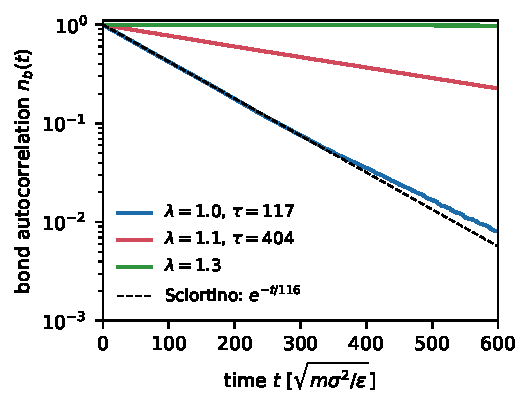
\includegraphics[width=0.48\textwidth]{figures/dumbbells.pdf}\hfill
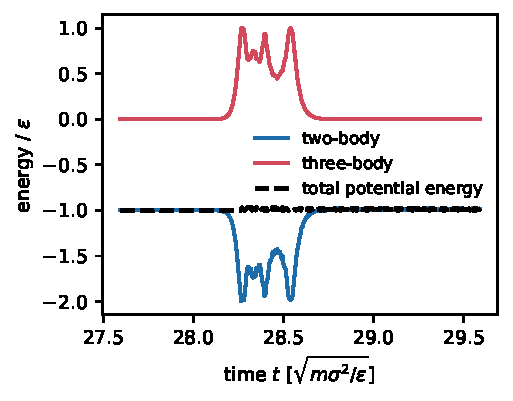
\includegraphics[width=0.48\textwidth]{figures/swap_event.pdf}
\caption{Left: bond autocorrelation of the dumbbell system for $\lambda = 1$, 1.1 and 1.3, with the
reference decay $e^{-t/116}$ of Ref.~\cite{Sciortino2017}. Right: energies during a burst of bond
swaps of one A and two B particles ($n=150$, $\lambda=1$, NVE, $kT\approx0.01$); the two-body and
three-body energies compensate and the total potential energy stays at $-\epsilon$.}
\label{fig:dumbbells}
\end{figure}

\subsection{Potential energy during a swap event}

One A and two B particles move in NVE in a box of side 2.6 ($n = 150$, $\lambda = 1$,
\texttt{examples/\allowbreak dumbbells/\allowbreak in.swap\_event}). During a swap, the two-body energy drops to $-2\epsilon$
while the three-body energy rises to $+\epsilon$, so the potential energy stays at $-\epsilon$
(Fig.~\ref{fig:dumbbells}, right). The total energy is conserved to $10^{-5}$ over $1.5\times10^5$
steps.

\subsection{Kremer--Grest sticker network}

A melt of 200 Kremer--Grest chains of 20 beads with stickers at beads 2, 6, 10, 14 and 18
(\cmd{examples/kg\_network}) is first turned into a dissociative network: stickers form and break
bonds with $E_\text{bond} = -24\epsilon$ at $kT = 1$, and the number of bonds settles at about 400 of
500 possible (Fig.~\ref{fig:kg}, left). With formation and breaking switched off, the number of bonds
is conserved (409 bonds before and after $2\times10^5$ steps for every barrier) and the shift and
swap moves relax the topology. The barrier enters as the gate $e^{-E_a/kT}$: going from $E_a = 0$ to
$2\epsilon$ and $4\epsilon$ reduces the number of attempts by factors of 7.40 and 7.33 per step of
$2kT$ and the number of accepted exchanges by 7.45 and 7.2, close to $e^2 = 7.39$. The bond
autocorrelation time grows from $\tau_x = 128\tau$ to $739\tau$ and about $4300\tau$ (the last value
extrapolated beyond the run), a factor of 5--6 per $2kT$, because exchanges that swap a bond back
restore the original pairing (Fig.~\ref{fig:kg}, right).

\begin{figure}[h]
\centering
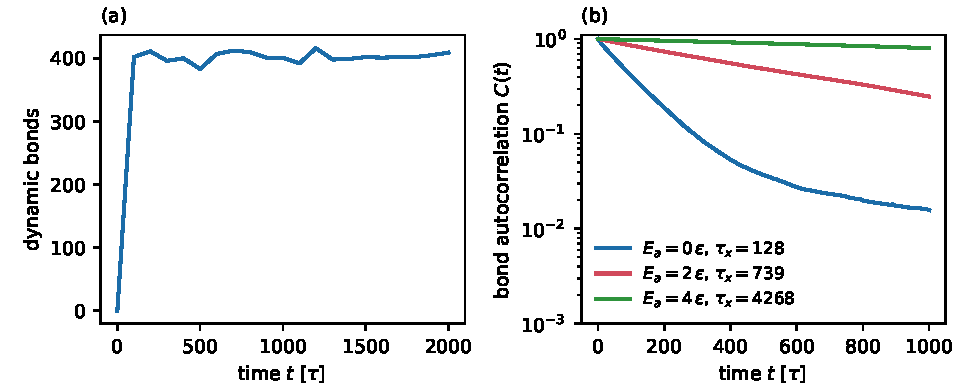
\includegraphics[width=0.9\textwidth]{figures/kg_network.pdf}
\caption{Left: number of dynamic bonds during reversible formation and breaking. Right: bond
autocorrelation in the same network with exchange only, for three barriers.}\label{fig:kg}
\end{figure}

%======================================================================
\section{Notes on other implementations}

These were found while comparing BondFlux with the codes and papers it builds on:
\begin{itemize}
\item \cmd{pair\_style lj3b} of the 3b-potentials package omits the factor $1/r^2$ in its
  two-body and three-body forces, so the force is $r^2$ times $-\partial E/\partial r$;
  \cmd{fs3b} of the same package is consistent.
\item HOOMD-blue 7.2.0 RevCross: correct forces and virial; the three-body energy is not included
  in the potential energy (Table~\ref{tab:hoomd}).
\item MC\_exchange 1.3.0: the sub-domain bounds of its neighbor list assume a box starting at 0;
  sites with three or more bonded pairs are skipped; the lowest-energy candidate is chosen
  deterministically; \cmd{alpha} scales $\Delta E$; and \cmd{P\_coeff}$>1$ breaks detailed balance.
\item TICG binary vitrimer code: the swap move checks the reaction radius for the new partner only.
\item Ref.~\cite{Xia2024b}: barrier inside the Metropolis exponent (Sec.~\ref{sec:rules});
  Ref.~\cite{Xia2023}: window checked for the new bond only.
\end{itemize}

\begin{thebibliography}{99}
\bibitem{Montarnal2011} D. Montarnal, M. Capelot, F. Tournilhac, L. Leibler, Science \textbf{334}, 965 (2011).
\bibitem{Ducrot2014} E. Ducrot, Y. Chen, M. Bulters, R. P. Sijbesma, C. Creton, Science \textbf{344}, 186 (2014).
\bibitem{Kremer1990} K. Kremer, G. S. Grest, J. Chem. Phys. \textbf{92}, 5057 (1990).
\bibitem{Perego2020} A. Perego, F. Khabaz, Macromolecules \textbf{53}, 8406 (2020).
\bibitem{Xia2023} J. Xia, J. A. Kalow, M. Olvera de la Cruz, Macromolecules \textbf{56}, 8080 (2023).
\bibitem{Xia2024b} J. Xia, M. Olvera de la Cruz, Macromolecules \textbf{57}, 8793 (2024).
\bibitem{Sciortino2017} F. Sciortino, Eur. Phys. J. E \textbf{40}, 3 (2017).
\bibitem{Ciarella2019} S. Ciarella, W. G. Ellenbroek, arXiv:1912.08569 (2019).
\bibitem{Anderson2020} J. A. Anderson, J. Glaser, S. C. Glotzer, Comput. Mater. Sci. \textbf{173}, 109363 (2020).
\bibitem{Lin2026} M.-H. Lin, T.-W. Lin, C. E. Sing, J. Chem. Phys. \textbf{164}, 144908 (2026).
\bibitem{Zhao2022} H. Zhao, X. Wei, Y. Fang, K. Gao, T. Yue, L. Zhang, V. Ganesan, F. Meng, J. Liu,
  Macromolecules \textbf{55}, 1091 (2022).
\end{thebibliography}

\end{document}
